\section{Metric distances}

Vector spaces, even when equipped with (weighted) $L_p$-norms, lack the generality required to handle the diverse range of feature types and distance functions essential for multimedia (MM) data.

\paragraph*{Metric spaces}
A metric space $M = (U,d)$ is defined as a pair, where:
\begin{itemize}
    \item $U$ represents a domain of values.
    \item $d$ is a distance function that, for all $x, y, z \in U$, satisfies the metric axioms:
        \begin{itemize}
            \item \textit{Positivity}: $D(x,y) \geq 0, D(x,y) = 0 \leftrightarrow x = y$.
            \item \textit{Symmetry}: $D(x,y) = D(y,x)$. 
            \item \textit{Triangle inequality}: $D(x,y) \leq D(x,z) + D(z,y)$. 
        \end{itemize}
\end{itemize}
All the distance functions previously discussed, as well as the (weighted) $L_p$-norms, adhere to the metric axioms. 
Metric indexes leverage these axioms to organize objects and utilize the triangle inequality for search space pruning.

\paragraph*{Shape matching}
Consider two sets of points, $S_1$ and $S_2$:
\begin{figure}[H]
    \centering
    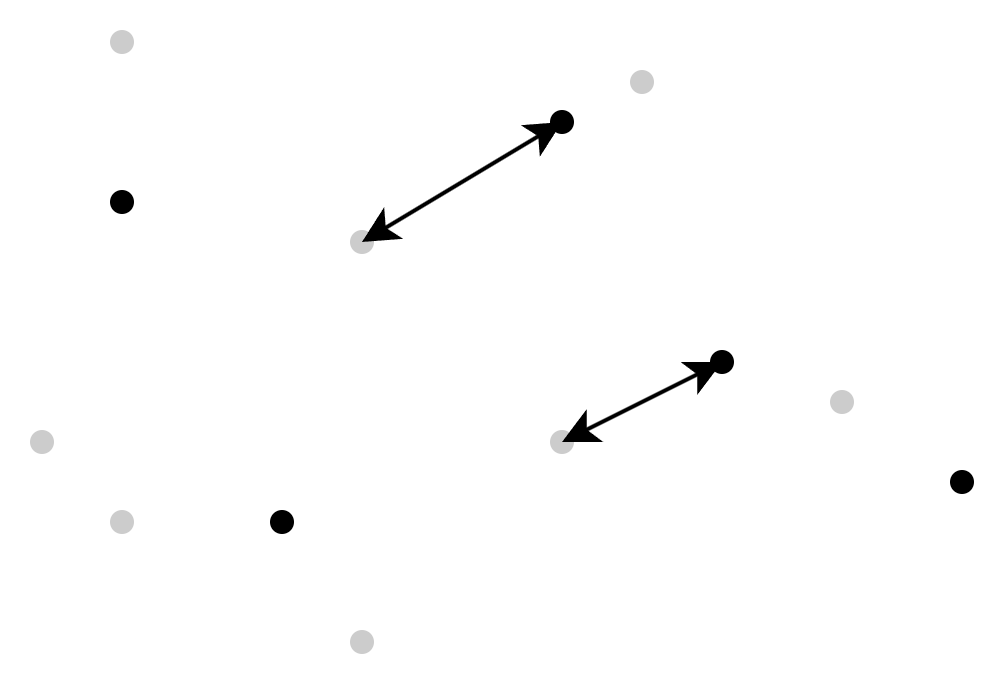
\includegraphics[width=0.5\linewidth]{images/hd.png}
\end{figure}
The Hausdorff distance is defined through the following steps:
\begin{enumerate}
    \item For each gray point in $S_1$, find the closest black point in $S_2$. 
        Let $h(S_1,S_2)$ be the maximum of these distances.
    \item For each black point in $S_2$, find the closest gray point in $S_1$. 
        Let $h(S_2,S_1)$ be the maximum of these distances.
    \item Compute the Hausdorff distance as:
        \[\text{D}_{\text{Haus}}(S_1,S_2) = \max\{ h(S_1,S_2),h(S_2,S_1)\}\]
\end{enumerate}
This technique is particularly useful for matching shapes.

\paragraph*{Set similarity}
To calculate the difference and similarities between two sets, $s_1$ and $s_2$, the function $D_{setdiff}(s_1,s_2)$ can be employed: 
\[D_{setdiff}(s_1,s_2)=\dfrac{\left\lvert s_1 - s_2 \right\rvert \left\lvert s_2 - s_1 \right\rvert }{\left\lvert s_1 \left\lvert +\right\rvert s_2 \right\rvert}\]

\paragraph*{Edit distance}
The edit distance is a commonly used measure for strings, defined as the minimum number of operations required (insertions, deletions, or substitutions) to transform one string $s_1$ into another string $s_2$. 
\begin{example}
    Consider the following pairs: 
    \begin{enumerate}
        \item $\left\langle \text{ball},\text{bull} \right\rangle$.
        \item $\left\langle \text{balls},\text{bell} \right\rangle$.
        \item $\left\langle \text{rather},\text{alter} \right\rangle$.
    \end{enumerate}
    The corresponding edit distances are: 
    \begin{enumerate}
        \item $D_{\text{edit}}(\text{ball},\text{bull})=1$.
        \item $D_{\text{edit}}(\text{balls},\text{bell})=2$.
        \item $D_{\text{edit}}(\text{rather},\text{alter})=3$.
    \end{enumerate}
\end{example}
The edit distance is widely used in genomic databases to compare DNA sequences. 
Each DNA sequence is treated as a string over the 4-letter alphabet of bases.
\begin{example}
    Consider the pair $\left\langle \text{rather},\text{alter} \right\rangle$. 
    The edit distance computation involves two matrices. 
    Initially, the cost matrix is defined as follows:
    \begin{table}[H]
        \centering
        \begin{tabular}{c|c|c|c|c|c|c|}
        \hline
        \multicolumn{1}{|c|}{\textbf{r}} & 1         & 1          & 1          & 1          & 1          & 0          \\ \hline
        \multicolumn{1}{|c|}{\textbf{e}} & 1         & 1          & 1          & 1          & 0          & 1          \\ \hline
        \multicolumn{1}{|c|}{\textbf{h}} & 1         & 1          & 1          & 0          & 1          & 1          \\ \hline
        \multicolumn{1}{|c|}{\textbf{t}} & 1         & 1          & 1          & 1          & 1          & 1          \\ \hline
        \multicolumn{1}{|c|}{\textbf{a}} & 1         & 0          & 1          & 1          & 1          & 1          \\ \hline
        \multicolumn{1}{|c|}{\textbf{r}} & 1         & 1          & 1          & 1          & 1          & 0          \\ \hline
        \multicolumn{1}{|c|}{$\uparrow$}& 0         & 1          & 1          & 1          & 1          & 1          \\ \hline
                                         & $\rightarrow$ & \textbf{a} & \textbf{l} & \textbf{t} & \textbf{e} & \textbf{r} \\ \cline{2-7} 
        \end{tabular}
    \end{table}
    This matrix is utilized to incrementally construct the new matrix $D_{\text{edit}}$, with its elements recursively defined as:
    \[D_{\text{edit}}^{(i,j)}=\text{cost}_{(i,j)}+\min\left\{D_{\text{edit}}^{(i-1,j)},D_{\text{edit}}^{(i,j-1)},D_{\text{edit}}^{(i-1,j-1)}\right\}\]
    In this case, the resulting table is as follows:
    \begin{table}[H]
        \centering
        \begin{tabular}{c|c|c|c|c|c|c|}
        \hline
        \multicolumn{1}{|c|}{\textbf{r}}          & 6                      & 5          & 5          & 5          & 4          & 3          \\ \hline
        \multicolumn{1}{|c|}{\textbf{e}}          & 5                      & 4          & 4          & 4          & 3          & 4          \\ \hline
        \multicolumn{1}{|c|}{\textbf{h}}          & 4                      & 3          & 3          & 3          & 3          & 4          \\ \hline
        \multicolumn{1}{|c|}{\textbf{t}}          & 3                      & 2          & 3          & 2          & 3          & 4          \\ \hline
        \multicolumn{1}{|c|}{\textbf{a}}          & 2                      & 1          & 2          & 3          & 4          & 5          \\ \hline
        \multicolumn{1}{|c|}{\textbf{r}}          & 1                      & 1          & 2          & 3          & 4          & 4          \\ \hline
        \multicolumn{1}{|c|}{$\uparrow$}          & 0                      & 1          & 2          & 3          & 4          & 5          \\ \hline
                                                  & $\rightarrow$          & \textbf{a} & \textbf{l} & \textbf{t} & \textbf{e} & \textbf{r} \\ \cline{2-7} 
        \end{tabular}
    \end{table}
\end{example}

\paragraph*{Fréchet distance}
The Fréchet distance, also known as the dog-keeper distance, serves as a superior measure of similarity between curves compared to the Hausdorff distance. 
This metric finds application in diverse fields such as speech recognition, signature and handwriting recognition, as well as the matching of time series and the analysis of moving objects.
Consider an individual moving along a finite path while walking a dog on a leash, each following a distinct finite path. 
The Fréchet distance quantifies the length of the shortest leash required for both the person and the dog to traverse their respective paths entirely.

\paragraph*{Metric indexing principles}
Given a metric dataset $P \subseteq U$, it can be partitioned into two subsets using one of the following principles:
\begin{enumerate}
    \item \textit{Ball decomposition}: start with a designated point $v$, referred to as the vantage point. 
        Calculate the distances of all other points $p$ in relation to $v$, denoted as $D(p,v)$. 
        Then, define two subsets as follows:
        \[P_1=\{p|D(p,v)\leq r_v\}\]
        \[P_2= \{p|D(p,v)>r_v\}\]
        For a given range query ${p|D(p,q)\leq r}$, if $D(q,v)>r_v+r$, it can be inferred that no point in $P_1$ belongs to the result. 
        Similar reasoning applies to $P_2$.
    \item \textit{Generalized hyperplane}: choose two points, $v_1$ and $v_2$. 
        Compute the distances of all other points $p$ with respect to both $v_1$ and $v_2$.     
        Define two subsets as follows:
        \[P_1=\{p|D(p,v_1)\leq D(p,v_2)\}\]
        \[P_2=\{p|D(p,v_2)<D(p,v_1)\}\]
        For a range query $\{p|D(p,q)\leq r\}$, if $D(q,v_1)-D(q,v_2)>2r$, it implies that no point in $P_1$ contributes to the result.
\end{enumerate}

\subsection{M-tree}
The M-tree ha been the inaugural dynamic, paged, and balanced metric index, extending the principles of R-trees to arbitrary metric spaces.
At a glance, the M-tree bears a resemblance to an R-tree. 
Nevertheless, it exclusively operates with distance values, disregarding coordinate values, and abstains from relying on any geometric reasoning.

\paragraph*{Structure}
Objects are recursively aggregated in a bottom-up manner based on regions in a structure where regions are allowed to overlap. 
Each node, except the root, can house up to $C_{\text{max}}$ entries, with a minimum requirement of $C_{\text{min}} \leq 0.5\cdot C_{\text{max}}$

Each tree node $N$ is associated with a region, denoted as $\text{Reg}(N)$, defined by:
\[\text{Reg}(N)=\{p|p\in U,D(p,v_N) \leq r_N\}\]
Here, $v_N$ (referred to as the "center") is also known as a routing object, and $r_N$ is termed the covering radius of the region. 
The set of indexed points $p$ reachable from node $N$ ensures that $D(p,v_N) \leq r_N$. 
This allows the application of the pruning principle: if $D(q,v_N)>r_N+r$, then prune node $N$.

In leaf nodes, an entry $E$ in node $N$ takes the form $E=\left\langle \text{ObjFeatures}, \text{distP}, \text{RID} \right\rangle $, where ObjFeatures represent the feature values of the indexed object, and distP is the distance between the object and its parent routing object (i.e., the routing object of node $N$).

For internal nodes, an entry $E$ in node $N$ is expressed as:
\[E=\left\langle \text{RoutingObjFeatures}, \text{CoveringRadius}, \text{distP}, \text{PID} \right\rangle \]
Here, RoutingObjFeatures encompass the feature values of the routing object, CoveringRadius denotes the radius of the region, and distP represents the distance between the routing object and its parent routing object (undefined for entries in the root node).

\paragraph*{Characteristics}
During query execution, pre-computed distances, denoted as distP, are leveraged to conserve computational resources.
Let $v_P$ represent the parent routing object of $v_N$.
When examining the entry of $v_N$, the distance $D(q,v_P)$ between the query and its parent has already been computed. 
Consequently, we have knowledge of the distance $D(v_P,v_N)$.
Applying the triangle inequality, we can deduce that:
\[D(q,vN) \geq \left\lvert  D(q,v_P) - D(v_P,v_N)\right\rvert\]
This allows us to prune node $N$ without computing $D(q,v_N)$ if:
\[\left\lvert D(q,v_P) - D(v_P,v_N)\right\rvert > r_N + r\]

\paragraph*{Operations}
The process of inserting a new object relies on a Penalty method. 
This method evaluates the increment in the covering radius required to incorporate the new object. 
When handling a split, there are various alternatives, including:
\begin{itemize}
    \item \texttt{mM\_RAD}: minimize the maximum of the two resulting radii.
    \item \texttt{M\_LB\_DIST}: choose the closest and farthest objects from $v_N$.
\end{itemize}
Experiments reveal that \texttt{mM\_RAD} yields the best results.